% Document class `report-template` accepts either project-plan or final-report option in
% []. This will change the title page as necessary.
\documentclass[project-plan]{report-template}
% \documentclass[final-report]{report-template}

% Packages I use in my report.
\usepackage{graphicx}
\usepackage{amsmath}
\usepackage{blindtext}
\usepackage{float}
\usepackage{booktabs}   % toprule / midrule / bottomrule
\usepackage{tabularx}   % auto-wrapping columns to a fixed width
\usepackage{ragged2e}
\usepackage{caption}
\usepackage{hyperref}
% Utilizing APA replacing bibtex backend with biber
\usepackage[style=apa,backend=biber]{biblatex}
\addbibresource{references.bib} % Replacing the old bibliography file loading


% Directory where I saved my figures.
\graphicspath{{./figures/}}

% Metadata used for the title page - please modify.
\university{Imperial College London}
\department{Department of Earth Science and Engineering}
\course{MSc in Renewable Energy with Data Science \& AI: Geology \& Geophysics}
\title{Resilient Coastlines: A Multi-Layered Predictive Framework for Mangrove Monitoring in Guyana}
\author{Zuriel Mbonde}
\email{zuriel.mbonde25@imperial.ac.uk}
\githubusername{esemsc-mm123}
\supervisors{Dr. Temitope D. Timothy Oyedotun\\
             Dr. James Percival}
\repository{https://github.com/ese-ada-lovelace-2025/irp-zam25}

% Left-aligned, ragged-right auto-wrapping column
\newcolumntype{L}{>{\RaggedRight\arraybackslash}X}

\begin{document}

\maketitlepage  % generate title page

\section*{AI Acknowledgment Statement}
I used Anthropic's Claude Opus 4.8 (\url{https://claude.ai/}) to pressure-test some of my ideas, particularly Objective 3, and teach me unfamiliar concepts. I also used the same version of Claude to clarify ideas and terminology in remote-sensing after reading several papers during my initial research. Finally, I made use of Claude's LaTeX abilities to help generate the template for a table and citation. The contents were filled with dummy text that I replaced without the use of AI. Generative AI was not used to create nor edit any text on this project plan. The submitted work reflects my own understanding. Any AI-assisted preliminary ideas suggested to me were corroborated with literature, re-derived and written in my own words. 

% Abstract
\section*{Abstract}
Mangrove monitoring plays a key role in assessing coastal defense vulnerabilities, particularly for densely populated coastal areas below sea level. In Guyana, mangroves are threatened by erosional cycles and anthropogenic factors, leading to significant losses. This paper employs remote sensing techniques and machine learning to evaluate L-band SAR to improve its accuracy in predicting mangrove extent. This study also formulates a coastal flooding risk index which includes fringe width, tree structure and spectral indexes. The risk index is then used for sensitivity analysis and hindcasting the Dantzig-Fairfield seawall breach. This research sets the stage as a methodology to uncover early-warning indicators of coastal flooding. This may help institutions like the National Agricultural Research and Extension Institute (NAREI) and international bodies better prepare for increasing climate-change induced risk factors and partake in coastal resilience initiatives. 

% Introduction section
\section{Introduction}
Ninety percent of Guyana’s population reside on a low-lying coastal plain that is at or below sea level \parencite{Oyedotun2025, Pelling1999}. Historically this has put communities, wildlife and farmland at risk of coastal flooding \parencite{Lakhan1994}. The man-made cemented seawall, originally introduced by the Dutch and British in the 1880s, has allowed for the coastal strip to be reclaimed \parencite{Bassett2013}. Beyond the sea-facing wall, naturally occurring mangroves are situated in the intertidal zones often characterized by mudflats and salt marshes \parencite{Best2022}. Mangroves are widely regarded as a natural defense against rising tides and coastal waves \parencite{Hernandez2024, Van2023, Blankespoor2017}. As a “first line of defense” followed by a seawall, this mangrove-led hybrid infrastructure reduces the inundation risk \parencite{De2023}. Along Guyana’s 430 km coast, mangroves are in decline. Between 2023 and 2024, there was a net loss of 1478 hectares in mangrove cover \parencite{Narei2024}. Natural causes such as erosion and increased volatility due to mud bank migration have increased the rate of degradation \parencite{Dookie2022}. Anthropogenic factors like pollution and urbanization resulting in coastal squeezing also play a role in their reduction \parencite{Johnson2018}. Despite restoration efforts, \textcite{Narei2024} underscores bolstering mangrove protection and rehabilitation efforts as a necessity.
\vspace{5 mm}

The spatiotemporal mapping of mangroves is a key component to understanding the dynamics affecting mangroves and where intervention can be exercised \parencite{Pimple2025, Spalding2014}. Remote sensing techniques involving satellite optical data combined with supervised machine learning such as Random Forests (RF) classifiers have produced precise mangrove extent maps \parencite{Fallatah2026, Elmahdy2020}. \textcite{Nedd2023} uses optical data (Landsat) and Synthetic Aperture Radar (SAR) to train a RF to map the change in Guyana’s mangrove canopy coverage. Landsat is classified, vector-clipped and used to bound the classification of PALSAR HV for earlier years \parencite{Nedd2023}. Post 2016, Landsat is fused with SAR Sentinel-1C. \textcite{Chan2024} compares Sentinel-1C Band, Sentinel-2, Landsat and their fusion as inputs into a RF model trained on a 2018 mangrove extent dataset from NAREI. The fusion model of all datasets showed the highest overall accuracy (95\%), user accuracy (69\%), and producer accuracy (87\%) \parencite{Chan2024}. Sentinel-1C lagged behind with a 28.6\% F1 Score compared to 93\%+ for the other isolated datasets. Evaluating both studies, the fusion of PALSAR HV/HH (L-band) has yet to be studied. Given its longer wavelength compared to Sentinel-1C (C-band), it can penetrate canopies and inform on woody mangrove structures like stem density, potentially increasing the level of user and producer accuracy \parencite{Saatchi2019}.
\vspace{5 mm}

Methods in risk assessment are also influential drivers in mangrove protection and restoration initiatives. \textcite{Liu2026} derives a comprehensive health index taking into account tree characteristics like root spread to canopy diameter, root length per unit area and boring density as a weighted sum. Given the study takes individual tree samples across sites, remote sensing techniques would involve measuring lagging health/stress proxies (as opposed to early-warning indicators) such as Normalized Difference Vegetation Index (NDVI) for mangrove patches from optical data \parencite{Liu2026}. Evaluating the role of fringe width as a key characteristic of a mangrove forest’s wave attenuating ability reported in \textcite{Best2022}, a weighted sum can be formulated to map vulnerable areas of the mangrove belt where there’s a higher risk of coastal flooding. \textcite{Xu2024} posits a mangrove coastal protection index as a weighted product including fringe width, canopy height and NDVI. However, a weighted sum may cover a wider range of possible scenarios when conducting Monte Carlo simulations for sensitivity analysis. The issue of coarse resolution canopy height data may also be resolved using L-band SAR HH/HV for tree structure in the coastal protection index.
\vspace{5 mm}

Hindcasting may be useful to understand how flood risk models detect patterns leading up to a significant flood event. Region Five of Guyana’s coast has suffered from a major sea-wall breach in Dantzig and Fairfield in 2019. Coastal erosion due to spring high tides and a depleted mangrove defense were said to be the main drivers \parencite{DailyHerald2019}. Given a stable extent map model without retraining, the question emerges as to whether the risk-layered model could retroactively predict a pattern of growing vulnerability pre-2019. How did each component change in that time window, controlling tide and seasonality? Which indicator most consistently mirrored patterns of failure associated with the event? Questions like these may help to determine the importance of these risk factors as early warning signs of failure in coastal defense.
\vspace{5 mm}

This paper attempts to use publicly available satellite imagery from the Google Earth Engine (GEE) data catalogue to address the following objectives:

\begin{enumerate}
    \item Evaluate the role of L-band SAR HH/HV as an additive technique to improve the accuracy of mangrove extent mapping compared to the \textcite{Chan2024} benchmark.
    \item Devise a coastal flooding risk index using the extent map produced and evaluate the importance of these risk factors along the six coastal regions of Guyana
    \item Develop a hindcast using the existing classifier to examine the ability of the risk index to measure patterns of failure leading up to the 2019 Dantzig-Fairfield seawall breach.
\end{enumerate}

% Another section
\section{Methodology}
The first step in building a mangrove extent map is data collection. Sentinel-2 and Landsat 2 will be selected for their multispectral bands which can be extracted and used for imaging vegetation. Spectral indices like NDVI, which utilize near infrared (NIR) and red (RED) bands can be calculated to help detect mangrove patches. Fusing both optical datasets rather than employing them in isolation is typically encouraged as it increases revisit times \parencite{Claverie2018}. This is crucial in tropical nations like Guyana with heavy cloud coverage. \textcite{Chan2024} shows how cloud-free images increase significantly with a combined dataset. L-band SAR as an additional dataset to this fusion with optical and Sentinel-C SAR may complement well since HH/HV SAR backscatter is cloud independent. Besides its deep canopy penetration ability mentioned earlier, L-band SAR may improve detecting inundated canopies due to its longer wavelength \parencite{Meyer2019}. This is often a challenge with mapping mangrove during high tide. After preprocessing optical and SAR respectively, determining band ratios like NDVI shown in eq~\ref{eq:ndvi}, and training a RF model on 2020 WorldCover v100 dataset, extent maps will be inferred for 2021. High-resolution Google Earth imagery and the 2021 WorldCover v200 will be used to compare the accuracy with the \textcite{Chan2024} benchmark. Correspondence is currently ongoing with researchers to obtain the same training and validation set used in their study.
% NDVI Equation
\begin{equation}
    \label{eq:ndvi}
    NDVI = \frac{NIR - RED}{NIR + RED}
\end{equation}

Using the 2021 inferred extent maps as a mask, a coastal flooding risk map can be produced taking into account health/stress proxies like NDVI and Salinity Index (SI) in eq.~\ref{eq:si}, calculating fringe width from shoreline-normal transects and determining tree structure from volume scattering attributed to HH/HV SAR backscatter. This index would resemble a weighted sum whose sensitivity would be analyzed from a monte carlo simulation. Alternatives include manually perturbed weights based on expert recommendations which may be computationally cheap but less likely to capture complex non-linear relationships. One caveat associated with this index is that it doesn’t include the state of the seawall and the engineering dynamics undergirded.

% SI Equation
\begin{equation}
    \label{eq:si}
    SI = \frac{B3 + B4}{B2}
\end{equation}
where $B2 = Blue$, $B3 = Green$, and $B4 = Red$ 

Given a trained mangrove extent model layered with a risk gradient from derived weights for the Dantzig and Fairfield region, each index indicator can be tracked from 2017 until the spring of 2019. This may uncover trends and correlations, informing their role in describing the 2019 sea-wall breach. This hindcast is favored over a long-term forecasting method to deepen links between objectives and make use of the validation event that typically justifies the need for healthy mangroves in the context of coastal flood resilience.

To achieve each of the project objectives, various datasets will be employed for various time windows in correspondence with the validating data as shown in Table ~\ref{tab:datasets}.

\begin{table}[H]
\centering
\caption{Summary of datasets, sources, time covered, methods, and objectives covered.}
\label{tab:datasets}
\small
\begin{tabularx}{\textwidth}{%
  >{\hsize=0.9\hsize}L%   Dataset
  >{\hsize=0.9\hsize}L%   Source
  >{\hsize=0.8\hsize}L%   Time covered
  >{\hsize=1.5\hsize}L%   Methodology
  >{\hsize=0.9\hsize}L%   Objectives covered
}
\toprule
\textbf{Dataset} & \textbf{Source} & \textbf{Time} & \textbf{Methodology} & \textbf{Objectives} \\
\midrule
\href{https://developers.google.com/earth-engine/datasets/catalog/COPERNICUS_S1_GRD}{Sentinel-1 SAR C-band} & European Union/ESA/Copernicus & 2020-2021 & Extent mapping & O1 \\
\addlinespace
\href{https://developers.google.com/earth-engine/datasets/catalog/COPERNICUS_S2_SR_HARMONIZED}{Sentinel-2 Harmonized, Atmosphere Corrected} & European Union/ESA/Copernicus & 2017-2019 2020-2021  & Extent mapping, risk index calculation, hindcasting & O1, O2, O3 \\
\addlinespace
\href{https://developers.google.com/earth-engine/datasets/catalog/LANDSAT_LC08_C02_T1_L2}{Landsat 8 Atmosphere Corrected} & USGS & 2017-2019 2020-2021 & Extent mapping, risk index calculation, hindcasting & O1, O2, O3 \\
\addlinespace
\href{https://developers.google.com/earth-engine/datasets/catalog/JAXA_ALOS_PALSAR_YEARLY_SAR_EPOCH}{ALOS PALSAR SAR L-band} & JAXA EORC & 2017-2019  2020--2021 & Extent mapping, risk index calculation, hindcasting &  O1, O2, O3 \\
\addlinespace
\href{https://developers.google.com/earth-engine/datasets/catalog/ESA_WorldCover_v100}{ESA WorldCover 10m v100} & ESA WorldCover Consortium & 2020-2021 & Extent mapping training labels &  O1 \\
\addlinespace
\href{https://developers.google.com/earth-engine/datasets/catalog/ESA_WorldCover_v200}{ESA WorldCover 10m v200} & ESA WorldCover Consortium & 2021-2022 & Extent mapping validation labels & O1 \\
\bottomrule
\end{tabularx}
\end{table}

\section{Future Plan}
The following in Figure~\ref{fig:gantt} is a Gantt chart detailing the project timeline.
% Figure
\begin{figure}[H]
    \begin{center}
        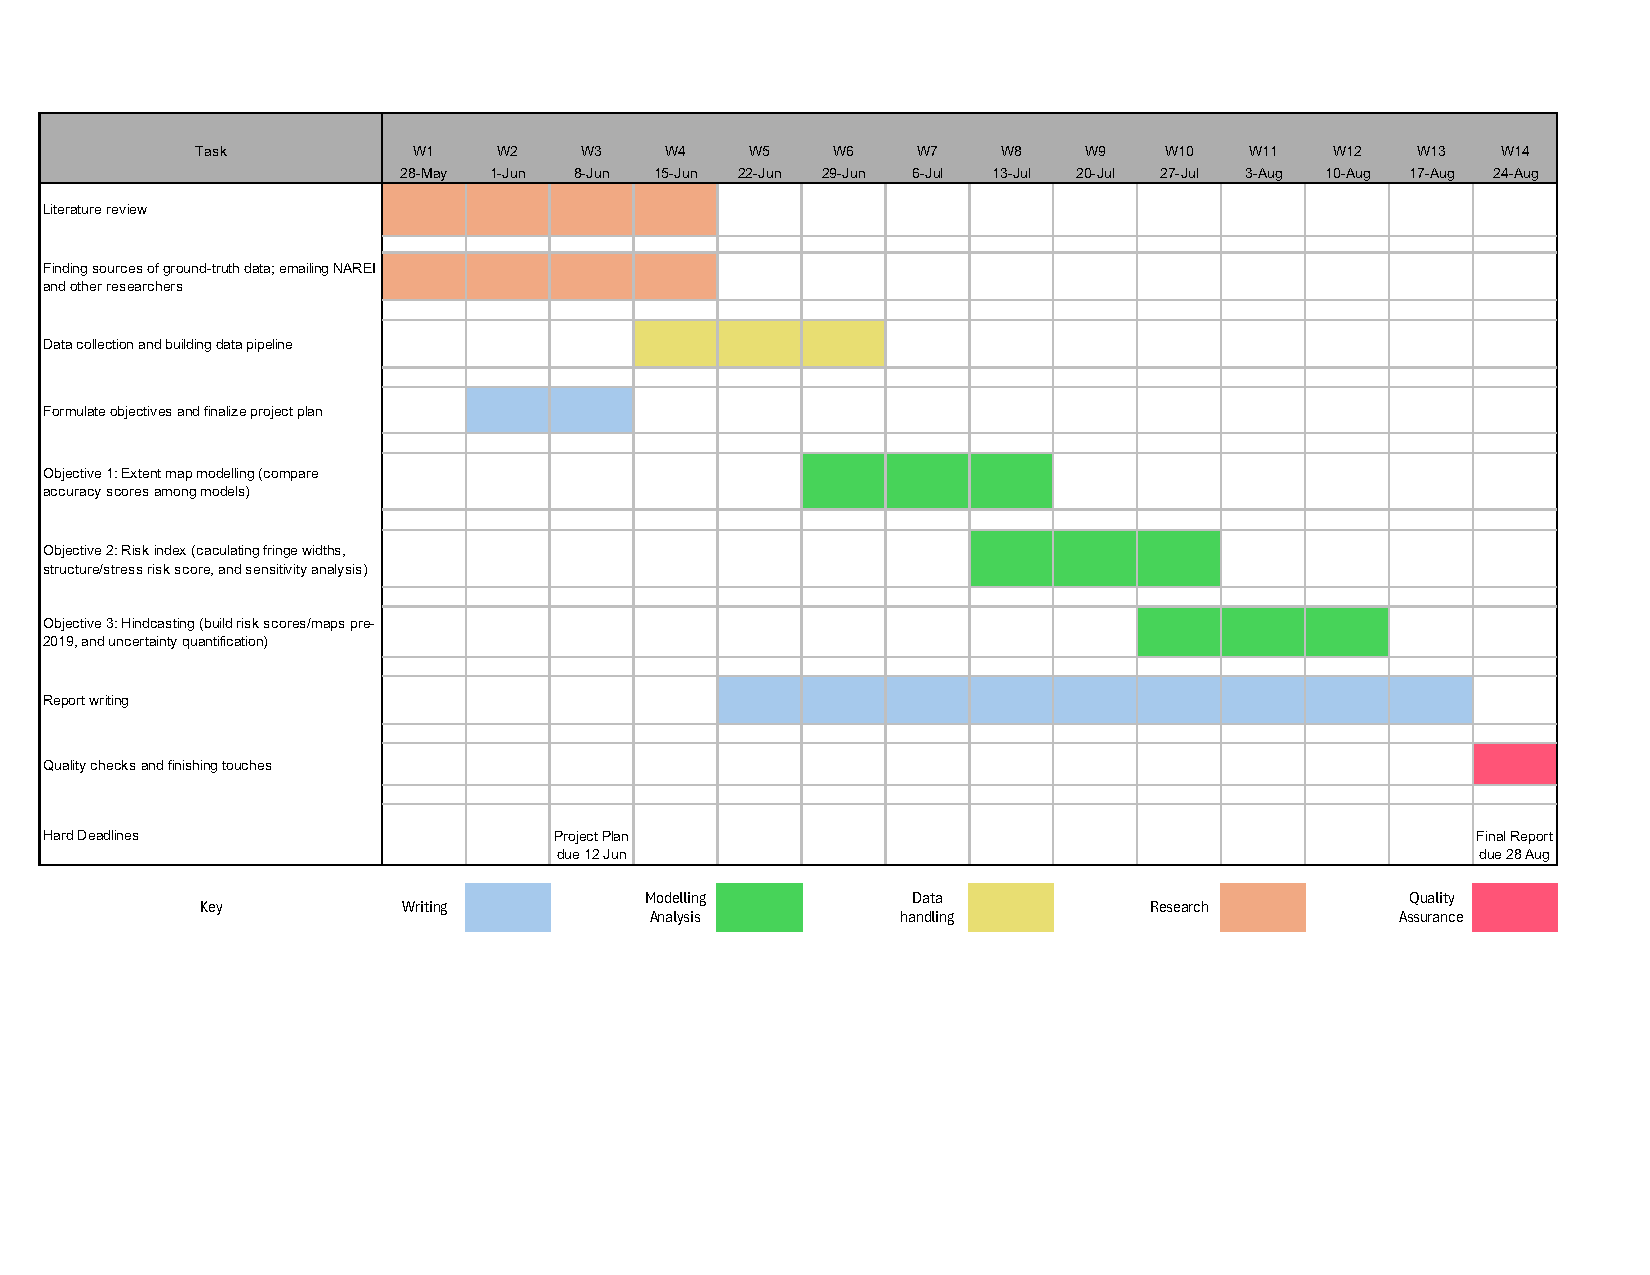
\includegraphics[width=1.1\textwidth]{figures/IRP Gantt Chart.pdf}
    \end{center}
    \vspace{-0.8cm} 
    \caption{\label{fig:gantt} A Gantt Chart showing the work to be done}
\end{figure}

% References
\printbibliography

\end{document}          
